% !TEX root = submission.tex
% This contents of this file will be inserted into the _Solutions version of the
% output tex document.  Here's an example:

% If assignment with subquestion (1.a) requires a written response, you will
% find the following flag within this document: <SCPD_SUBMISSION_TAG>_1a
% In this example, you would insert the LaTeX for your solution to (1.a) between
% the <SCPD_SUBMISSION_TAG>_1a flags.  If you also constrain your answer between the
% START_CODE_HERE and END_CODE_HERE flags, your LaTeX will be styled as a
% solution within the final document.

% Please do not use the '<SCPD_SUBMISSION_TAG>' character anywhere within your code.  As expected,
% that will confuse the regular expressions we use to identify your solution.

\def\assignmentnum{6 }
\def\assignmentname{Bayesian Networks}
\def\assignmenttitle{XCS221 Assignment \assignmentnum --- \assignmentname}
\input{macros}
\begin{document}
\pagestyle{myheadings} \markboth{}{\assignmenttitle}

% <SCPD_SUBMISSION_TAG>_entire_submission

This handout includes space for every question that requires a written response.
Please feel free to use it to handwrite your solutions (legibly, please).  If
you choose to typeset your solutions, the |README.md| for this assignment includes
instructions to regenerate this handout with your typeset \LaTeX{} solutions.
\ruleskip

\LARGE
1.a
\normalsize

% <SCPD_SUBMISSION_TAG>_1a
\begin{answer}
  % ### START CODE HERE ###
  $\text{Rain} \rightarrow \text{WetGrass}$

  $\text{Sprinkler} \rightarrow \text{WetGrass}$
  % ### END CODE HERE ###
\end{answer}
% <SCPD_SUBMISSION_TAG>_1a

\LARGE
1.b
\normalsize

% <SCPD_SUBMISSION_TAG>_1b
\begin{answer}
  % ### START CODE HERE ###
  $\mathbb{P}(\text{Rain}, \text{Sprinkler}, \text{WetGrass}) = p(\text{Rain}) \cdot p(\text{Sprinkler}) \cdot p(\text{WetGrass} \mid \text{Rain}, \text{Sprinkler})$
  % ### END CODE HERE ###
\end{answer}
% <SCPD_SUBMISSION_TAG>_1b

\LARGE
1.c
\normalsize

% <SCPD_SUBMISSION_TAG>_1c
\begin{answer}
  % ### START CODE HERE ###
  \[
    \mathbb{P}(\text{WetGrass}) = \sum_{r \in \{\text{T},\text{F}\}} \sum_{s \in \{\text{T},\text{F}\}} p(\text{Rain}=r) \cdot p(\text{Sprinkler}=s) \cdot p(\text{WetGrass} \mid \text{Rain}=r, \text{Sprinkler}=s)
  \]
  % ### END CODE HERE ###
\end{answer}
% <SCPD_SUBMISSION_TAG>_1c

\LARGE
1.d
\normalsize

% <SCPD_SUBMISSION_TAG>_1d
\begin{answer}
  % ### START CODE HERE ###
  \begin{align*}
    &\mathbb{P}(\text{Rain}=\text{T}, \text{Sprinkler}=\text{T}, \text{WetGrass}=\text{F}) \\
    &= p(\text{Rain}=\text{T}) \cdot p(\text{Sprinkler}=\text{T}) \cdot p(\text{WetGrass}=\text{F} \mid \text{Rain}=\text{T}, \text{Sprinkler}=\text{T}) \\
    &= 0.2 \times 0.5 \times (1 - 0.9) \\
    &= 0.2 \times 0.5 \times 0.1 = \mathbf{0.01}
  \end{align*}
  % ### END CODE HERE ###
\end{answer}
% <SCPD_SUBMISSION_TAG>_1d

\LARGE
1.e
\normalsize

% <SCPD_SUBMISSION_TAG>_1e
\begin{answer}
  % ### START CODE HERE ###
  \begin{enumerate}[label=(\alph*)]
    \item \textbf{True.} Rain and Sprinkler have no edge between them and no common ancestor, so they are marginally independent.
    \item \textbf{False.} Conditioning on WetGrass (a common child/collider) activates the path Rain $\rightarrow$ WetGrass $\leftarrow$ Sprinkler, causing explaining-away: the two variables become dependent.
    \item \textbf{True.} If we learn the sprinkler was on, it partially explains the wet grass, making Rain less probable than it would be given only WetGrass.
  \end{enumerate}
  % ### END CODE HERE ###
\end{answer}
% <SCPD_SUBMISSION_TAG>_1e
\clearpage

\LARGE
2.d
\normalsize

% <SCPD_SUBMISSION_TAG>_2d
\begin{answer}
  % ### START CODE HERE ###
  Output of \texttt{test\_forward\_sampling()} with \texttt{mutation\_rate=0.1}, \texttt{genome\_length=10}, seeds 123:

  \begin{center}
  \begin{tabular}{|l|l|}
  \hline
  \textbf{Species} & \textbf{Genome} \\
  \hline
  Thomas bayus      & T T C C A T T C C C \\
  Humblus studentus & T G C C A T T C C T \\
  Aryamus bayus     & T T C C A T T C C C \\
  Kenius bayus      & T T C C A T T C C C \\
  \hline
  \end{tabular}
  \end{center}

  Joint probability: $5.5 \times 10^{-11}$ (i.e.\ \texttt{0.0000000055\%})
  % ### END CODE HERE ###
\end{answer}
% <SCPD_SUBMISSION_TAG>_2d

\LARGE
2.g
\normalsize

% <SCPD_SUBMISSION_TAG>_2g
\begin{answer}
  % ### START CODE HERE ###
  Estimating $\mathbb{P}(\text{ThomasBayus}=\text{AAAC} \mid \text{KeniusBayus}=\text{AAAA})$
  with \texttt{mutation\_rate=0.1}, \texttt{genome\_length=4}:

  \begin{center}
  \begin{tabular}{|l|c|l|}
  \hline
  \textbf{Method} & \textbf{Steps/Iterations} & \textbf{Estimated Posterior} \\
  \hline
  Rejection sampling & 100      & 0.0000 \\
  Rejection sampling & 10{,}000 & 0.0000 \\
  Gibbs sampling     & 100      & 0.0900 \\
  Gibbs sampling     & 10{,}000 & 0.0332 \\
  Exact              & ---      & 0.0335 \\
  \hline
  \end{tabular}
  \end{center}

  Rejection sampling gets 0 because the evidence (Kenius=AAAA) occurs with probability $\approx 0.25^4 \approx 0.4\%$, so very few samples are accepted and none happen to have Thomas=AAAC. Gibbs sampling converges close to the exact value even with 10{,}000 iterations because it conditions on the evidence directly and mixes efficiently.
  % ### END CODE HERE ###
\end{answer}
% <SCPD_SUBMISSION_TAG>_2g
\clearpage

\LARGE
3.a
\normalsize

% <SCPD_SUBMISSION_TAG>_3a
\begin{answer}
  % ### START CODE HERE ###
  $Y \rightarrow A_1$

  $Y \rightarrow A_2$

  $Y \rightarrow A_3$
  % ### END CODE HERE ###
\end{answer}
% <SCPD_SUBMISSION_TAG>_3a

\LARGE
3.b
\normalsize

% <SCPD_SUBMISSION_TAG>_3b
\begin{answer}
  % ### START CODE HERE ###
  \begin{center}
  \begin{tabular}{|c|c|c|}
  \hline
  $Y$ & $p(A_1 = \text{good} \mid Y)$ & $p(A_1 = \text{bad} \mid Y)$ \\
  \hline
  $\text{good}$ & 1.0 & 0.0 \\
  $\text{bad}$  & 0.0 & 1.0 \\
  \hline
  \end{tabular}
  \end{center}
  % ### END CODE HERE ###
\end{answer}
% <SCPD_SUBMISSION_TAG>_3b

\LARGE
3.c
\normalsize

% <SCPD_SUBMISSION_TAG>_3c
\begin{answer}
  % ### START CODE HERE ###
  \begin{center}
  \begin{tabular}{|c|c|c|}
  \hline
  $Y$ & $p(A_1 = \text{good} \mid Y)$ & $p(A_1 = \text{bad} \mid Y)$ \\
  \hline
  $\text{good}$ & 0.5 & 0.5 \\
  $\text{bad}$  & 0.5 & 0.5 \\
  \hline
  \end{tabular}
  \end{center}
  % ### END CODE HERE ###
\end{answer}
% <SCPD_SUBMISSION_TAG>_3c

\LARGE
3.g
\normalsize

% <SCPD_SUBMISSION_TAG>_3g
\begin{answer}
  % ### START CODE HERE ###
  \textbf{Annotator A\_2 is the least trustworthy.}

  From the MLE-trained CPT plot (\texttt{plots/annotators.png}):
  \begin{itemize}
    \item A\_0: $p(\text{good} \mid Y=\text{good}) \approx 0.90$, $p(\text{bad} \mid Y=\text{bad}) \approx 0.87$ --- high accuracy.
    \item A\_1: $p(\text{good} \mid Y=\text{good}) \approx 0.85$, $p(\text{bad} \mid Y=\text{bad}) \approx 0.87$ --- high accuracy.
    \item A\_2: $p(\text{good} \mid Y=\text{good}) \approx 0.63$, $p(\text{bad} \mid Y=\text{bad}) \approx 0.53$ --- close to random (0.5).
  \end{itemize}

  A\_2's CPT is nearly uniform regardless of the ground-truth label, meaning its annotations carry almost no information about the true label. A\_0 and A\_1 are strongly diagonal (they agree with the ground truth most of the time), whereas A\_2 barely beats random guessing.
  % ### END CODE HERE ###
\end{answer}
% <SCPD_SUBMISSION_TAG>_3g
\clearpage

\LARGE
4.d
\normalsize

% <SCPD_SUBMISSION_TAG>_4d
\begin{answer}
  % ### START CODE HERE ###
  After running \texttt{test\_em\_learn()} for 100 iterations:

  \textbf{Annotator CPTs} (\texttt{plots/annotators\_em.png}):

  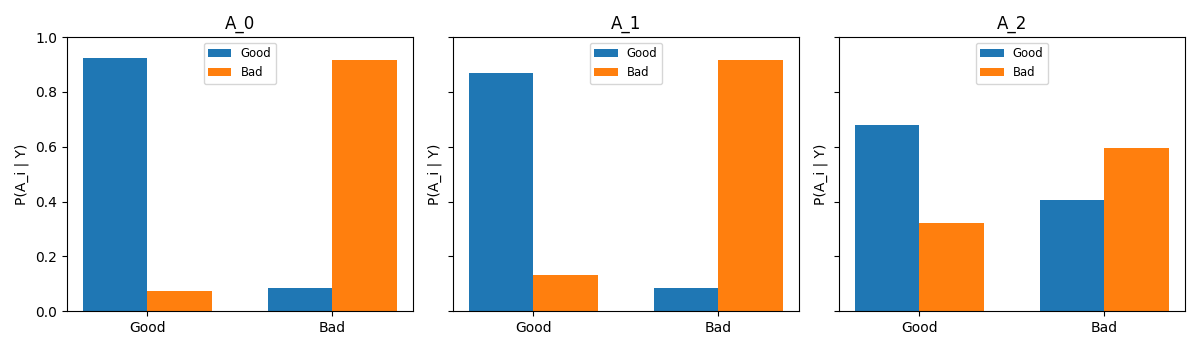
\includegraphics[width=\textwidth]{../src/plots/annotators_em.png}

  \textbf{Label posteriors} (\texttt{plots/labels\_em.png}):

  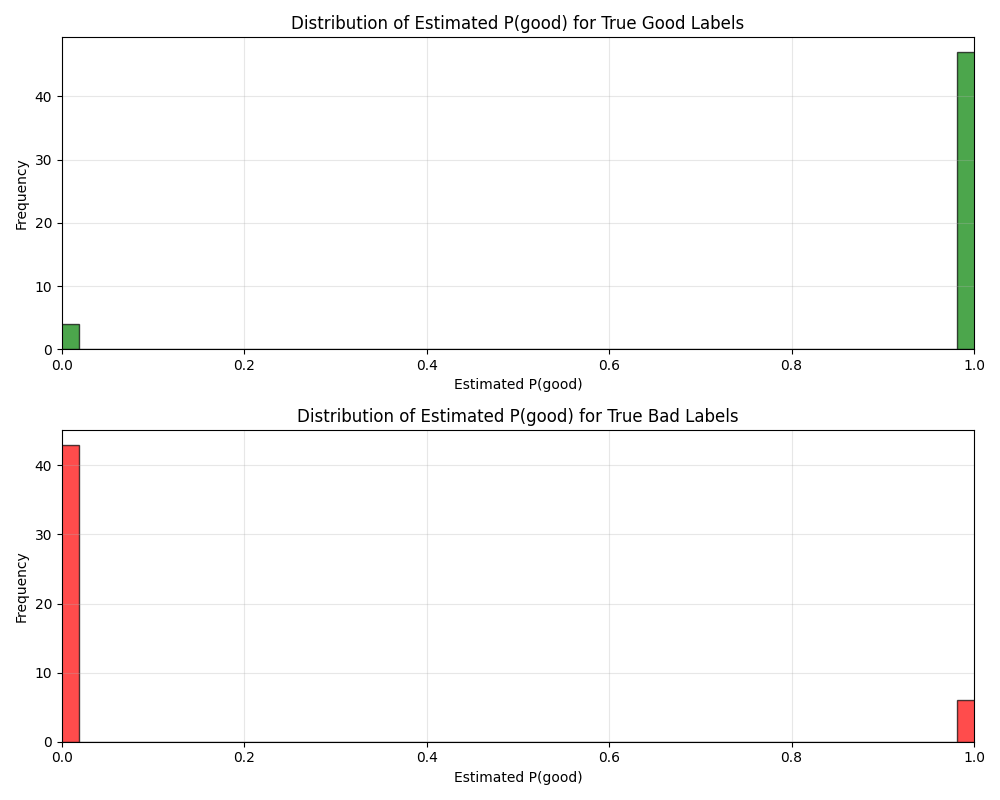
\includegraphics[width=0.8\textwidth]{../src/plots/labels_em.png}
  % ### END CODE HERE ###
\end{answer}
% <SCPD_SUBMISSION_TAG>_4d

\LARGE
4.e
\normalsize

% <SCPD_SUBMISSION_TAG>_4e
\begin{answer}
  % ### START CODE HERE ###
  \textbf{Yes}, the EM algorithm largely recovered the true labels.

  Evidence from \texttt{plots/labels\_em.png}:
  \begin{itemize}
    \item \textbf{Top histogram} (true good labels): the vast majority of data points with ground-truth label ``good'' receive an estimated $P(\text{good}) \approx 1.0$ from EM, with only a handful near 0.
    \item \textbf{Bottom histogram} (true bad labels): the vast majority of data points with ground-truth label ``bad'' receive an estimated $P(\text{good}) \approx 0.0$, with only a handful near 1.
  \end{itemize}

  This bimodal separation shows that EM confidently assigns high posterior probability to the correct label for most data points, even though no ground-truth labels were provided during training. The small number of misclassified points correspond to ambiguous data points where annotators disagreed.
  % ### END CODE HERE ###
  \end{answer}
% <SCPD_SUBMISSION_TAG>_4e

\clearpage


\LARGE
5.a
\normalsize

% <SCPD_SUBMISSION_TAG>_5a
\begin{answer}
  % ### START CODE HERE ###
  \textbf{Product: Claude Code (Anthropic)}

  Claude Code is an AI coding assistant that automates tasks such as writing boilerplate, debugging, code review, test generation, documentation, and entire feature implementation from natural-language descriptions. The jobs most directly in scope include junior and mid-level software engineers, QA engineers, technical writers, and code reviewers. A 2024 McKinsey Global Institute report (\textit{The economic potential of generative AI}) projects that software development is among the top three functions most affected by generative AI, with 20--45\% of developer time on routine coding tasks potentially automated in the near term.

  From an ecosystem perspective, Claude Code required substantial upstream human labor to build and maintain: large-scale data labeling and curating of code repositories, human feedback collection (RLHF annotators who rated code quality and safety), infrastructure engineers running GPU clusters, and ongoing policy and trust-and-safety reviewers who screen model outputs. This ``hidden'' labor force---often contracted at lower wages and in different geographies---enabled the product but is largely invisible to end users.
  % ### END CODE HERE ###
\end{answer}
% <SCPD_SUBMISSION_TAG>_5a

\LARGE
5.b
\normalsize

% <SCPD_SUBMISSION_TAG>_5b
\begin{answer}
  % ### START CODE HERE ###
  Claude Code currently sits closer to \textbf{augmentation} than direct displacement: it requires an engineer to review, validate, and integrate its suggestions, and it struggles with large-scale architectural reasoning and novel algorithmic design. In practice, it reduces the time skilled developers spend on routine tasks, raising their effective output rather than eliminating their roles. However, the displacement risk is real for entry-level positions: tasks that used to require a junior engineer (writing CRUD endpoints, generating unit tests) can now be completed by a senior engineer with Claude Code in a fraction of the time, reducing the need to hire juniors.

  The risks of incorrect augmentation include: (1) \textbf{over-reliance}---developers accepting subtly buggy or insecure code without careful review, increasing production vulnerabilities; (2) \textbf{skill atrophy}---engineers who rely on AI for boilerplate may lose the ability to write such code themselves, making them fragile when the tool is unavailable or wrong; and (3) \textbf{legal/IP exposure}---generated code may inadvertently reproduce licensed content, creating liability for employers.
  % ### END CODE HERE ###
\end{answer}
% <SCPD_SUBMISSION_TAG>_5b

\LARGE
5.c
\normalsize

% <SCPD_SUBMISSION_TAG>_5c
\begin{answer}
  % ### START CODE HERE ###
  Claude Code's subscription cost (\$20+/month) and English-language optimization mean it primarily benefits developers at well-funded companies in high-income countries, potentially \textbf{widening} the productivity gap between resource-rich and resource-constrained teams. Developers in lower-income regions or open-source communities who cannot afford the API costs are left at a compounding disadvantage---those who most need productivity boosts may have the least access. Conversely, making capable coding tools more affordable could narrow the gap between solo developers in emerging markets and large engineering teams, if the pricing model were adjusted.

  Performance disparities deepen inequality beyond access: Claude Code has been documented to perform better on common languages (Python, JavaScript) than on niche or regional languages (e.g., Erlang, languages prominent in non-Western ecosystems). Engineers working in those ecosystems get a worse product at the same price. Metrics that should be monitored include code acceptance rates and error rates stratified by programming language, geographic region of the user, and organization size, along with user-reported satisfaction across these groups.
  % ### END CODE HERE ###
\end{answer}
% <SCPD_SUBMISSION_TAG>_5c

\LARGE
5.d
\normalsize

% <SCPD_SUBMISSION_TAG>_5d
\begin{answer}
  % ### START CODE HERE ###
  A pragmatic mitigation strategy is a mandated \textbf{human-in-the-loop review gate} for AI-generated code in production systems, combined with employer-funded reskilling programs. Concretely, organizations using Claude Code for production deployments would be required (or incentivized by insurers/auditors) to have a licensed engineer review and sign off on AI-generated changes before merging, preserving meaningful human agency and accountability. This reduces the risk of silent vulnerabilities from unreviewed AI output and creates a continuing need for human engineering judgment.

  To address displacement at the junior-engineer level, companies that deploy AI coding assistants above a usage threshold could be required to contribute to an industry reskilling fund---analogous to apprenticeship levies in some European countries---that finances bootcamps and on-the-job training for displaced or aspiring engineers. Human oversight is central: the review gate ensures engineers remain active participants rather than passive rubber-stampers, while the reskilling programs ensure the labor market can adapt to the new division of work between humans and AI systems.
  % ### END CODE HERE ###
\end{answer}
% <SCPD_SUBMISSION_TAG>_5d
\clearpage

\LARGE
6.a
\normalsize

% <SCPD_SUBMISSION_TAG>_6a
\begin{answer}
  % ### START CODE HERE ###
  \textbf{Summary.} Claude Code is a terminal-based AI coding agent that can read, write, and execute code across an entire repository. Its strengths are deep context awareness (it can reason about a whole codebase at once), strong natural-language instruction following, and safe-by-default behavior that asks for confirmation before destructive actions. Its main weaknesses are high subscription cost that excludes many potential users, uneven performance across programming languages, limited ability to reason about long-horizon architectural decisions, and opacity around training data and model internals that makes it hard for users to understand or predict failure modes.

  \textbf{Improvements.} First, I would introduce a \textit{tiered pricing model}---a free tier limited to a reasonable monthly token budget and open-source project use, reducing the access gap for students, researchers, and developers in lower-income regions. Second, I would add a \textit{structured audit log} that records every AI-suggested change with its rationale, enabling teams to retrospectively review AI contributions and satisfying compliance requirements in regulated industries. Third, I would invest in systematic evaluation benchmarks stratified by programming language and domain so that performance gaps are publicly disclosed, allowing users to make informed decisions about where to trust the tool and motivating targeted improvements in underserved language ecosystems.
  % ### END CODE HERE ###
\end{answer}
% <SCPD_SUBMISSION_TAG>_6a

\LARGE
6.b
\normalsize

% <SCPD_SUBMISSION_TAG>_6b
\begin{answer}
  % ### START CODE HERE ###
  Currently, the power to shape Claude Code rests primarily with Anthropic's \textbf{engineers and executives}: they decide what data to train on, what safety constraints to impose, how to price access, and what capabilities to expose. Policymakers exert limited direct influence, and users---while able to provide feedback---have no structural leverage over model updates or pricing. This concentration of power in a single private company creates tension with the societal interest in a broadly beneficial, equitably distributed tool.

  From a normative standpoint, meaningful responsibility should be distributed more broadly: \textbf{affected workers and labor representatives} should have input into deployment norms (e.g., whether AI-generated code must be labeled in code reviews); \textbf{independent auditors} should be able to inspect model behavior and training practices; and \textbf{policymakers} should set minimum transparency and access standards. A concrete recommendation is to require AI coding-tool providers above a revenue threshold to publish annual \textit{impact assessments}---analogous to environmental impact statements---documenting labor market effects, equity metrics, and security incident rates, giving the public the information needed to hold companies accountable.
  % ### END CODE HERE ###
\end{answer}
% <SCPD_SUBMISSION_TAG>_6b
\clearpage

% <SCPD_SUBMISSION_TAG>_entire_submission

\end{document}